\documentclass[10pt,a4paper]{article}
\usepackage[utf8]{inputenc}

% Define the page margin
\usepackage[margin=3cm]{geometry}

% Better typography (font rendering)
\usepackage{microtype}

% Math environments and macros
\usepackage{amsmath}
\usepackage{amsfonts}
\usepackage{amssymb}
\usepackage{amsthm}

% Define \includegraphics to include graphics
\usepackage{graphicx}

% Draw graphics from a text description
\usepackage{tikz}

% Syntax highlighting
\usepackage{minted}

% Set global minted options
\setminted{linenos, autogobble, frame=lines, framesep=2mm}

% Import the comment environment for orgtbl-mode
\usepackage{comment}

% Do not indent paragraphs
\usepackage{parskip}

\title{Operating Systems, Sheet 8}
\author{Marten Lienen (03670270)}

\begin{document}

\maketitle

\section*{Exercise 1}

\subsection*{Part 1.1)}

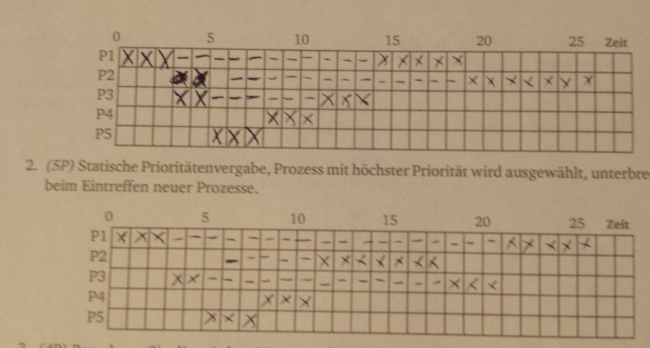
\includegraphics[width=\textwidth]{sheet-8/exercise-1-1}

\subsubsection*{Frage 3}

\begin{equation*}
  W_{1} = \frac{30}{5} = 6 \qquad W_{2} = \frac{36}{5} = 7.2
\end{equation*}

\subsection*{Part 1.2)}

\subsubsection*{Frage 1}

Der Dispatcher übernimmt den Austausch von rechnenden Prozessen und sorgt dafür, dass z.B. Register ordnungsgemäß gespeichert werden.
Der Scheduler ist derjenige, der bestimmt, welcher Prozess als nächstes vom Dispatcher geladen werden soll.

\subsubsection*{Frage 2}

Bei Prozessen muss alles ausgetauscht werden.
Bei Kernel-Level-Threads kann einiges gleichbleiben, sodass das Dispatchen von diesen etwas performanter ist.
Z.B. müssen Page Tables nicht getauscht werden, wenn die Threads zum selben Prozess gehören.
User-Level-Threads werden nicht vom Kernel gedispatcht sondern vom Programm selbst.
Dabei müssen generell dieselben Dinge gemacht werden wie beim Dispatching von Kernel-Threads, aber nicht vom Kernel.

\subsubsection*{Frage 3}

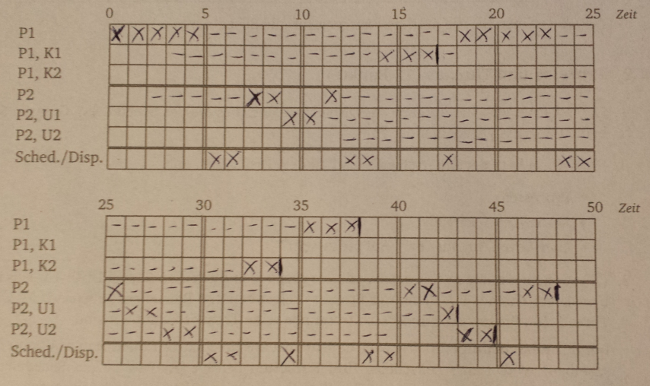
\includegraphics[width=\textwidth]{sheet-8/exercise-1-2-3}

\section*{Exercise 2}

\subsection*{Part 2.1)}

\begin{itemize}
\item Er terminiert (Die Berechnung ist beendet)
\item Der Benutzer fordert seine Beendigung
\item Ein nicht zu behandelnder Fehler tritt auf (z.B. Division durch 0)
\end{itemize}

\subsection*{Part 2.2)}

Ein Prozess der Priorität 3 kann dann laufen, wenn alle Threads mit höherer Priorität beendet sind oder warten.

\subsection*{Part 2.3)}

Es wird ungefähr 20ms dauern, weil der aktuelle Thread nur unterbrochen wird, wenn
\begin{itemize}
\item er terminiert
\item seine Zeitscheibe abläuft
\item er selbst IO macht
\end{itemize}

\subsection*{Part 2.4)}

Man könnte die Priorität unter die Basispriorität verringern, wenn ein Thread besonders viel Rechenzeit verbraucht hat, um das Aushungern anderer Prozesse und Threads zu verhindern.

\section*{Exercise 3}

\subsection*{Part 3.1)}

Der Heap ist ein großer, unorganisierter Haufen Speicher, auf dem man dynamisch Speicher reservieren kann.
Der Stack ist ein Stack, der die Argumente und Rücksprungadressen von Funktionsaufrufen speichert.

\subsection*{Part 3.2)}

Alle Stringfunktionen, die keine maximale Zeichenanzahl bekommen, sondern sich auf die Nullterminierung verlassen.

\subsection*{Part 3.3)}

Weil der Stack zu kleineren Adressen hinwächst, kann ein Angreifer Rücksprungadressen überschreiben, indem er z.B. dafür sorgt, dass ein String in eine zu kleine Stackvariable kopiert wird.
Dieser String enthält dann an der richtigen Stelle eine Adresse, die im Erfolgsfall in den String selbst zeigt und dort vom Angreifer vorbereiteten Code ausführt.

\subsection*{Part 3.4)}

Ein simpler Angriff, der den Zugriff gewährt ohne das Passwort zu kennen, ist
\begin{minted}{sh}
  $ ./auth $(echo -e -n \\0x1) 11111111111111111111
\end{minted}
Dabei schreibt man einfach direkt das Byte $1$ in die Variable result.
Allerdings funktioniert dies nur, wenn gewisse Schutzmechanismen gegen solche Angriffe beim Kompilieren deaktiviert werden.

Die Variable liegt auf dem Stack.

\subsection*{Part 3.5)}

Potentiell kann man dort auf dieselbe Weise Werte überschreiben, aber man kann darüber nicht direkt die Kontrolle übernehmen, und die Länge von Strings ist auch nicht direkt vorhersagbar.

\subsection*{Part 3.6)}

Einerseits sollte man immer die Längen von allen Variablen mitführen, um zu verhindern, dass an unerwünschte Positionen im Speichern geschrieben wird.
Gleichzeitig kann der Compiler solche Angriffe erschweren, indem er Adressen randomisiert.

\end{document}
